
\documentclass[conference]{IEEEtran}
\IEEEoverridecommandlockouts
\renewcommand{\thesection}{\Roman{section}}
\usepackage{booktabs}
\usepackage{fancyhdr}
\usepackage[usenames, dvipsnames]{xcolor}
\usepackage{colortbl}
\usepackage{caption}
\usepackage{graphicx}
\usepackage{array}
\usepackage{adjustbox}
\usepackage{hyperref,graphicx,color,float}
\definecolor{myblue}{RGB}{10, 150, 200}

\usepackage{cite}
\usepackage{multirow}
\usepackage{amsmath,amssymb,amsfonts}
\usepackage{algorithmic}
\usepackage{graphicx}
\usepackage{textcomp}
\usepackage{comment}
\definecolor{highlightColor}{HTML}{E6FFE6}

% --- packages required by this paper's figures and algorithm ---
\usepackage[ruled,vlined]{algorithm2e}
\usepackage{subcaption}
\usepackage{tikz}
\usetikzlibrary{positioning,arrows.meta,shapes.geometric,calc,fit,backgrounds}
\usepackage{pgfplots}
\pgfplotsset{compat=1.17}
\usepgfplotslibrary{groupplots}
\definecolor{beforeblue}{RGB}{31,119,180}
\definecolor{afterorange}{RGB}{255,127,14}

\usepackage{xcolor}
\def\BibTeX{{\rm B\kern-.05em{\sc i\kern-.025em b}\kern-.08em
    T\kern-.1667em\lower.7ex\hbox{E}\kern-.125emX}}

\pagestyle{plain}

\title{Entangled Enhancement in Modular Autonomous\\
Driving Systems: An Empirical Study of Cascade\\
Effects from Single-Component Retraining}

\author{\IEEEauthorblockN{Rashedul Arefin Ifty, Fumio Machida}
\IEEEauthorblockA{University of Tsukuba\\
Tsukuba, Japan\\
ifty.rashedul@sd.cs.tsukuba.ac.jp, machida@cs.tsukuba.ac.jp}}

\begin{document}
\maketitle
\bstctlcite{IEEEexample:BSTcontrol}% disable em-dash for repeated author names

\begin{abstract}
Machine learning systems in autonomous driving are maintained incrementally: one
component is retrained as its domain drifts while the rest of the pipeline stays
fixed. We study the downstream effect of such an update in a modular
perception--prediction--planning pipeline, built from a YOLOv11n detector (C1), a
constant-velocity predictor (C2), and a rule-based Intelligent Driver Model
planner (C3). We train C1 on Boston nuScenes scenes and fine-tune it on Singapore
scenes, measuring every component in two modes, \emph{isolated} with
ground-truth inputs and \emph{pipeline} with live upstream inputs. Rather than a
single retraining, we run a campaign of $15$ updates varying data size, training
length, and seed. Two effects related to the analytically modeled notion of
\emph{entangled enhancement} appear: a non-monotone cascade, in which an update
improves an interface yet worsens the plan, and a decoupling between a
component's aggregate metric and its interface behavior. The disruption is a
landscape rather than a constant, with the planned path moving between $1.33$ and
$7.80$~m. A further $12$ updates using a class-balanced training split remove the
small-data accuracy penalty and yield \emph{strict} entangled enhancement in
three cases, where the detector improves on its own metric while the planning
output degrades at the same time. Every isolated-mode metric remained
bit-identical, confirming that all changes propagated through the component
interfaces. Building on these findings we propose a cascade-aware retraining
assessment method and evaluate its low-cost interface-drift front-end, which
flags risky updates with a real but imperfect signal.
\end{abstract}

\begin{IEEEkeywords}
machine learning systems, autonomous driving, retraining, cascade effects,
software reliability, modular pipelines, regression testing
\end{IEEEkeywords}

% ============================================================================
\section{Introduction}
% ============================================================================
Autonomous driving systems are built either as a single end-to-end (E2E)
network that maps sensor input directly to a driving plan~\cite{chen2024e2esurvey,
hu2023uniad}, or as a modular pipeline of separately trained perception,
prediction, and planning components. In deployment, such systems are maintained
under domain drift one component at a time: a perception model is retrained for a
new city, a predictor is updated as agent statistics shift, a planner is revised
for new regulations. This component-scoped maintenance is only well-posed in a
modular pipeline, where components are separable and independently retrainable.
In an E2E model the smallest retrainable unit is the entire network, so we adopt
the modular pipeline as the setting for this study.

\looseness=-1
Retraining one component while the rest stay fixed is the common case in
practice, and it is also where a subtle hazard arises. This work
builds directly on Wang and Machida~\cite{wang2024compsac}, who model a
two-component MLS as a continuous-time Markov chain and name the failure mode
we study, \emph{entangled enhancement}: improving an upstream component on its
own metric can still degrade the system, because downstream components have
learned to operate on the previous upstream output. A follow-on study casts
this as an availability--continuity trade-off~\cite{wang2025issre}. Both are
stochastic models that need empirical calibration. So far no one has measured
how a single-component retraining event actually propagates through a real
perception--prediction--planning pipeline, nor how that propagation varies from
one retraining to the next. That is the gap this paper addresses.

\looseness=-1
The missing element is a controlled measurement of this propagation on a real
pipeline, and this paper supplies it. We build a three-component pipeline on
the nuScenes dataset~\cite{caesar2020nuscenes}: C1, a
YOLOv11n~\cite{jocher2024yolo11} camera detector, C2, a constant-velocity
trajectory predictor, and C3, a rule-based planner from the Intelligent Driver
Model (IDM) family~\cite{treiber2000idm} whose proposal-and-score design
follows PDM-Closed~\cite{dauner2023parting}. We train C1 on Boston scenes and
fine-tune it on Singapore scenes, a well-known domain gap within nuScenes,
keeping C2 and C3 frozen. The experiments center on two components. C1 is the
retrained unit, and C2 is its direct consumer. The interface between them, the
stream of detected objects, is where the cascade travels. C3 is kept as the
system-level readout that reports whether the change helps or harms the final
plan.

The main instrument is dual-mode evaluation, and it exists to separate a
component's own error from the error it inherits from upstream. Each downstream
component is measured twice: in \emph{isolated} mode with ground-truth inputs,
which exposes only its own error, and in \emph{pipeline} mode with live upstream
outputs, which exposes its own error plus whatever it inherits. The difference
between the two modes is the inherited part, so its change across a retraining
event measures the cascade that the retraining injects.

\looseness=-1
A single retraining, however, is one point. To learn whether the cascade is a
fixed property or a variable one, we run a \emph{campaign}: $15$ retraining
updates of C1 that vary the amount of fine-tuning data, the number of training
epochs, and the random seed, each measured through the same dual-mode harness.
This extends the study from a single observation to a landscape of retraining
outcomes, and it motivates a practical follow-up question: can a low-cost check,
computed from the detector's outputs alone, predict which updates disturb the
plan the most?

Our measurements yield seven findings, detailed in Section~\ref{sec:results}.
\begin{itemize}
\item[\textbf{F1.}] \textbf{(Architectural.)} The component-level retraining
question is unobservable in an E2E architecture and unaffordable at E2E training
costs; a modular pipeline is the enabling architecture.
\item[\textbf{F2.}] \textbf{(Isolation.)} The isolation property that stochastic
MLS models assume holds exactly: the isolated-mode metrics of the frozen C2 and
C3 stayed bit-identical across every retraining event.
\item[\textbf{F3.}] \textbf{(Cascade existence.)} Retraining C1 alone produced
large, measurable changes downstream, concentrated at the first C1$\to$C2
interface.
\item[\textbf{F4.}] \textbf{(Non-monotone cascade.)} An update can improve C2's
pipeline error yet worsen C3's planning error. In our reference run C2 improved
by 73.98\% while C3 worsened by 4.45\%.
\item[\textbf{F5.}] \textbf{(Metric decoupling.)} C1's aggregate mAP@50 can
\emph{drop} even as its outputs become more useful to C2, so a component's own
metric is not a reliable admission criterion.
\item[\textbf{F6.}] \textbf{(A landscape, not a constant.)} Across the $15$
updates the downstream disruption ranges widely (plan shift $1.33$--$7.80$~m),
the planner is hurt by most updates but helped by a few, and the effect grows
with fine-tuning data, so no single number summarizes the entanglement.
\item[\textbf{F7.}] \textbf{(Strict entangled enhancement.)} Once a
class-balanced fine-tune removes the small-data mAP penalty, $\delta_1$ turns
positive in $6$ of $12$ updates, and in $3$ of them the planner degrades at the
same time. This is the strict condition~\eqref{eq:ee}, observed here in a real
driving pipeline.
\end{itemize}

\textbf{Contributions.} This paper contributes (1)~a dual-mode measurement
method for retraining-induced cascades in modular MLS, with an isolation check;
(2)~a controlled measurement, to our knowledge the first on a real
perception--prediction--planning pipeline, of how single-component retraining
under a geographic domain shift propagates downstream, run as a $15$-update
campaign that reveals a non-monotone cascade, a decoupling between aggregate and
interface metrics, and a wide landscape of outcomes; and (3)~a cascade-aware
retraining assessment method (CARA) built on this measurement, whose
interface-drift front-end and admission rule we evaluate on the campaign.

The remainder of the paper is organized as follows.
Section~\ref{sec:method} formalizes the system model, including the definition
of entangled enhancement, and the dual-mode methodology.
Section~\ref{sec:cara} presents the proposed CARA method.
Section~\ref{sec:setup} details the experimental setup and the retraining
campaign. Section~\ref{sec:results} reports the evaluation results, both the
empirical entanglement findings and the evaluation of CARA.
Section~\ref{sec:related} reviews related work, and
Section~\ref{sec:conclusion} concludes.

% ============================================================================
\section{System Model and Methodology}
\label{sec:method}
% ============================================================================

\subsection{Formal Pipeline Model}
We model the driving stack as a composition of three functions,
\begin{equation}
S = C_3 \circ C_2 \circ C_1,
\qquad
S(x) = C_3\bigl(C_2(C_1(x))\bigr),
\label{eq:comp}
\end{equation}
where $x$ is a camera keyframe and the three components carry out the
canonical perception--prediction--planning decomposition:
\begin{itemize}
\item \textbf{C1 (Perception):} $z_1 = C_1(x)$ is a set of detected objects,
each with a class, a position, and an extent in the ego frame.
\item \textbf{C2 (Prediction):} $z_2 = C_2(z_1)$ is, for every detected
object, a forecast trajectory over the next several seconds.
\item \textbf{C3 (Planning):} $z_3 = C_3(z_2)$ is the ego vehicle's planned
trajectory, a sequence of positions over a $3$~s horizon.
\end{itemize}
The intermediate signals $z_1$ and $z_2$ are the pipeline interfaces, and each
is a cascade channel: a change in $C_1$'s output distribution shifts $z_1$,
which its direct consumer $C_2$ then propagates into $z_2$ and $C_3$.
Fig.~\ref{fig:pipeline} shows the pipeline annotated with the before/after
numbers from the reference retraining of this study. Only $C_1$ is retrained
(Boston $\to$ Singapore); the isolated (\emph{iso}) metrics of the frozen $C_2$
and $C_3$ stay constant, while their pipeline (\emph{pipe}) metrics move because
their inputs shift.

\begin{figure}[htbp]
\centering
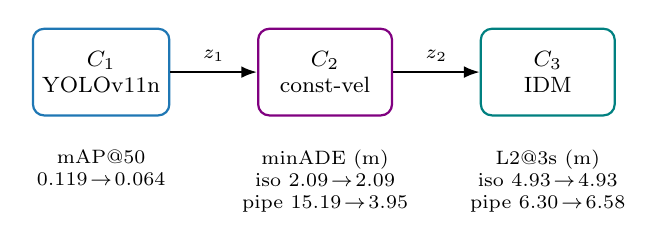
\begin{tikzpicture}[
    font=\footnotesize,
    comp/.style={draw, thick, rounded corners, minimum width=17mm,
                 minimum height=11mm, align=center},
    lbl/.style={align=center, font=\scriptsize},
    arr/.style={-{Latex[length=2mm]}, thick}
]
\node[comp, draw=beforeblue] (c1) {$C_1$\\YOLOv11n};
\node[comp, draw=violet, right=11mm of c1] (c2) {$C_2$\\const-vel};
\node[comp, draw=teal, right=11mm of c2] (c3) {$C_3$\\IDM};
\draw[arr] (c1) -- node[above,font=\scriptsize]{$z_1$} (c2);
\draw[arr] (c2) -- node[above,font=\scriptsize]{$z_2$} (c3);
\node[lbl, below=3mm of c1] {mAP@50\\$0.119\!\to\!0.064$};
\node[lbl, below=3mm of c2] {minADE (m)\\iso $2.09\!\to\!2.09$\\pipe $15.19\!\to\!3.95$};
\node[lbl, below=3mm of c3] {L2@3s (m)\\iso $4.93\!\to\!4.93$\\pipe $6.30\!\to\!6.58$};
\end{tikzpicture}
\caption{Pipeline $C_1\!\to\!C_2\!\to\!C_3$ with before/after numbers.}
\label{fig:pipeline}
\end{figure}

\subsection{Entangled Enhancement}
\label{sec:ee-def}
The failure mode this paper investigates is \emph{entangled enhancement}, named
by the stochastic MLS model of Wang and Machida~\cite{wang2024compsac}. In
words, an upstream component is retrained and improves on its own metric, yet
the system as a whole degrades, because downstream components were tuned to the
statistics of the \emph{previous} upstream output and are disturbed when that
output changes. Writing $\delta_1$ for the change in the C1 metric, with
positive $\delta_1$ denoting an improvement, and $\Delta_3$ for the change in
the terminal (planning) pipeline metric, with positive $\Delta_3$ denoting a
regression, the strict condition is
\begin{equation}
\underbrace{\delta_1 > 0}_{\text{C1 improves}}
\ \wedge\
\underbrace{\Delta_3 > 0}_{\text{system degrades}} .
\label{eq:ee}
\end{equation}
A closely related but weaker phenomenon is \emph{metric decoupling}: C1's
aggregate metric moves in the opposite direction to the usefulness of its
outputs to the downstream consumer, so $\delta_1 < 0$ while the C1$\to$C2
interface metric improves. Decoupling shows that a component's own score is an
unreliable proxy for its effect on the system, which is the same lesson as
entangled enhancement even when the strict sign condition~\eqref{eq:ee} is not
met. As Section~\ref{sec:results} reports, we observe both regimes. Small-data
fine-tuning drives $\delta_1 < 0$ across the main campaign, which yields
decoupling and non-monotone cascades, while a class-balanced fine-tune lifts
$\delta_1$ above zero and produces the strict condition~\eqref{eq:ee} itself.

\subsection{Dual-Mode Evaluation}
The core instrument is the measurement of each downstream component in two
modes. Let $z_k^{\star}$ denote the ground-truth value of interface $k$. In
\emph{isolated} mode a component receives ground-truth inputs, so for $C_2$ and
$C_3$ we evaluate
\begin{align}
z_2^{\text{iso}} &= C_2(z_1^{\star}), &
z_3^{\text{iso}} &= C_3(z_2^{\star}).
\label{eq:iso-mode}
\end{align}
In \emph{pipeline} mode a component receives the live output of its upstream
neighbor,
\begin{align}
z_2^{\text{pipe}} &= C_2(C_1(x)), &
z_3^{\text{pipe}} &= C_3(C_2(C_1(x))).
\label{eq:pipe-mode}
\end{align}
Isolated mode exposes a component's own error, and pipeline mode exposes its own
error plus the error inherited from upstream. For a component $C_k$ with error
metric $M_k$ (lower is better), the difference between the two is the inherited
part, which we call the \emph{cascade gap} at $C_k$,
\begin{equation}
\Gamma_k = M_k^{\text{pipeline}} - M_k^{\text{isolated}}.
\label{eq:gap}
\end{equation}
A retraining event $R$ applied to an upstream component changes the pipeline
metrics. If the system is properly modular, it leaves all isolated metrics of
untouched components unchanged. We call this the \emph{isolation property}:
\begin{equation}
M_k^{\text{isolated}}(\text{before } R) = M_k^{\text{isolated}}(\text{after } R)
\quad \forall \text{ frozen } C_k.
\label{eq:iso}
\end{equation}
Equation~\eqref{eq:iso} is not assumed but treated as a testable property of
the apparatus: any leakage of the retraining event into a frozen component's
isolated metric indicates contamination, and we verify the equation bit-exactly
in Section~\ref{sec:results}. The cascade \emph{injected} by $R$ at component
$C_k$ is then
\begin{equation}
\Delta_k = M_k^{\text{pipeline}}(\text{after } R) - M_k^{\text{pipeline}}(\text{before } R),
\label{eq:inj}
\end{equation}
which, given~\eqref{eq:iso}, equals the change in the cascade gap $\Gamma_k$.

\subsection{Cascade Diagnostic and Coupling Factor}
\label{sec:diag}
The canonical cascade hypothesis is a conjunction of three conditions: the
retrained upstream component improves on its own metric, the frozen terminal
component is stable in isolation, and it worsens in the pipeline. Using
$\delta_1$ and $\Delta_3$ from Section~\ref{sec:ee-def} and~\eqref{eq:inj}, we
encode the diagnostic as
\begin{equation}
\textsc{cascade} \equiv
\bigl(\delta_1 > 0\bigr)
\ \wedge\
\bigl(\Delta_3^{\text{iso}} = 0\bigr)
\ \wedge\
\bigl(\Delta_3 > \epsilon\bigr),
\label{eq:diag}
\end{equation}
with $\epsilon$ a small noise floor. When~\eqref{eq:diag} holds, the
coupling from the retrained component to the system output is summarized by
the \emph{cascade coupling factor}
\begin{equation}
\rho_{1\to 3} = \frac{\Delta_3}{\delta_1}.
\label{eq:rho-def}
\end{equation}
On a synthetic pipeline with a known planted cascade,
\eqref{eq:diag}--\eqref{eq:rho-def} recover $\rho_{1\to 3} \approx 0.84$, which
serves as an apparatus check prior to the empirical runs. As
Section~\ref{sec:results} shows, the empirical campaign does not satisfy the
conjunction~\eqref{eq:diag} in its canonical form, because $\delta_1 < 0$
throughout while $\Delta_3$ varies in sign, so $\rho_{1\to 3}$ is not cleanly
measurable and must be read together with the full cascade vector rather than as
an isolated scalar.

\subsection{Single-Component Retraining Under Domain Shift}
\label{sec:experiment}
Each retraining event follows the same procedure, and only C1 is ever changed:
\begin{enumerate}
\item Train C1 on the source domain (Boston scenes). Freeze C2 and C3
permanently.
\item Measure the five-quantity profile on the target-domain validation set
(Singapore): C1 detection quality (mAP@50), C2-isolated minADE, C2-pipeline
minADE, C3-isolated L2@$\{1,2,3\}$s, C3-pipeline L2@$\{1,2,3\}$s.
\item Fine-tune C1 on the target domain (Singapore scenes), producing the
retrained C1$'$.
\item Re-measure the identical five-quantity profile with C1$'$ in place.
\item Verify the isolation property~\eqref{eq:iso} and compute the injected
cascades~\eqref{eq:inj} at C2 and C3.
\end{enumerate}
The Boston-to-Singapore shift within nuScenes is a genuine and well-studied
domain gap: left- versus right-hand traffic, different vehicle and agent
mixes, and different lighting conditions~\cite{caesar2020nuscenes}.

\subsection{Metrics}
C1 is scored with standard detection metrics (mAP@50, mAP@50-95, precision,
recall) on the target-domain validation images. For $C_2$, the metric is the
minimum average displacement error (minADE). For an agent with forecast
positions $\hat{p}^{(m)}_{t}$ under mode $m$ and ground-truth positions
$p^{\star}_{t}$ over $T$ future steps,
\begin{equation}
\mathrm{minADE} = \min_{m}\ \frac{1}{T}\sum_{t=1}^{T}
\bigl\lVert \hat{p}^{(m)}_{t} - p^{\star}_{t} \bigr\rVert_2 ,
\label{eq:minade}
\end{equation}
averaged over agents. Our deterministic predictor has a single mode, so the
$\min$ collapses to that mode. For $C_3$, the metric is the L2 displacement
error between the planned ego trajectory $\hat{e}_t$ and the human driver's
recorded trajectory $e^{\star}_t$ at horizon $\tau$,
\begin{equation}
\mathrm{L2}@\tau = \bigl\lVert \hat{e}_{\tau} - e^{\star}_{\tau} \bigr\rVert_2 ,
\qquad \tau \in \{1,2,3\}\ \text{s},
\label{eq:l2}
\end{equation}
reported together with collision rate. We also report, for the campaign, a
\emph{plan shift}: the distance between the plan produced with the incumbent C1
and the plan produced with the retrained C1 on the same scene, which measures
how far a retraining moves the driving decision independent of the human path.
The L2 metric is the standard nuScenes open-loop planning protocol used by the
E2E literature~\cite{hu2023uniad,jiang2023vad,zhai2023rethinking}, with the
differential-use caveat discussed in Sections~\ref{sec:results} and
\ref{sec:related}.

% ============================================================================
\section{Cascade-Aware Retraining Assessment}
\label{sec:cara}
% ============================================================================
The measurement method of Section~\ref{sec:method} exposes a concrete hazard for
maintenance: a retrained component that regresses on its own metric may still
improve its neighbor while degrading the system, so neither component-level nor
first-interface validation is a sufficient admission criterion. We turn the
method into an admission check for component updates, Cascade-Aware Retraining
Assessment (CARA). CARA formalizes, as an explicit gate, the procedure we later
run across the campaign of Section~\ref{sec:setup}. Fig.~\ref{fig:cara}
summarizes the decision and Algorithm~\ref{alg:cara} states it. The evaluation of
CARA on real updates is deferred to Section~\ref{sec:results}.

\begin{figure}[htbp]
\centering
\resizebox{\columnwidth}{!}{%
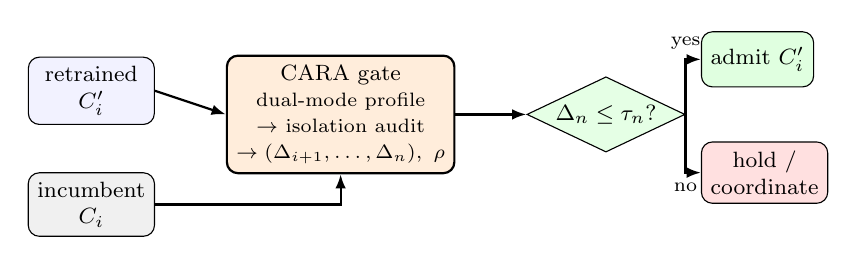
\begin{tikzpicture}[
    font=\footnotesize,
    node distance=5mm,
    box/.style={draw, rounded corners, minimum height=7mm, minimum width=16mm,
                align=center, fill=blue!5},
    old/.style={draw, rounded corners, minimum height=7mm, minimum width=16mm,
                align=center, fill=black!6},
    gate/.style={draw, rounded corners, minimum height=10mm, minimum width=26mm,
                 align=center, fill=orange!14, thick},
    dec/.style={draw, diamond, aspect=2.1, align=center, fill=green!10, inner sep=1pt},
    pass/.style={draw, rounded corners, minimum height=7mm, align=center, fill=green!12},
    stop/.style={draw, rounded corners, minimum height=7mm, align=center, fill=red!12},
    arr/.style={-{Latex[length=1.8mm]}, thick}
]
\node[box] (new) {retrained\\$C_i'$};
\node[old, below=6mm of new] (old) {incumbent\\$C_i$};
\node[gate, right=9mm of new, yshift=-3mm] (gate)
     {CARA gate\\\scriptsize dual-mode profile\\\scriptsize $\to$ isolation audit\\\scriptsize $\to (\Delta_{i+1},\dots,\Delta_n),\ \rho$};
\node[dec, right=9mm of gate] (dec) {$\Delta_n \le \tau_n$?};
\node[pass, above right=1mm and 7mm of dec] (pass) {admit $C_i'$};
\node[stop, below right=1mm and 7mm of dec] (stop) {hold /\\coordinate};
\draw[arr] (new.east) -- (gate.west);
\draw[arr] (old.east) -| ($(gate.south)$);
\draw[arr] (gate) -- (dec);
\draw[arr] (dec.east) |- (pass.west) node[midway,above,font=\scriptsize]{yes};
\draw[arr] (dec.east) |- (stop.west) node[midway,below,font=\scriptsize]{no};
\end{tikzpicture}%
}
\caption{The CARA admission check for a retrained component.}
\label{fig:cara}
\end{figure}

\subsection{The Admission Procedure}
Given a pipeline $C_1 \to \dots \to C_n$, a frozen audit set $A$, and a
candidate update $R$ to component $C_i$, CARA records the dual-mode profile with
the incumbent $C_i$, swaps in the retrained $C_i'$, and records it again on the
identical audit set with fixed randomness. It requires the isolation
property~\eqref{eq:iso} to hold for every frozen $C_k$. Any violation signals
leakage or nondeterminism and invalidates the assessment. In our campaign this
audit passed bit-exactly (F2). It then computes the injected cascade
$\Delta_k$~\eqref{eq:inj} at every downstream component and reports the full
vector $(\Delta_{i+1}, \dots, \Delta_n)$, because adjacent deltas can carry
opposite signs, together with the coupling factor $\rho_{i\to n} = \Delta_n /
\delta_i$. A negative $\rho$ with an improving $\delta_i$ is the
entangled-enhancement regime. As our campaign shows, $\rho$ is well-defined only
when $\delta_i$ is unambiguous. It is therefore not cleanly measurable on the
updates of Table~\ref{tab:campaign}, where $\delta_1 < 0$ throughout, but it is
well-posed on the class-balanced updates of Section~\ref{sec:res-balanced}, whose
detector metric moves definitely upward.
The update is admitted only if $\Delta_n \le \tau_n$ and safety-critical
auxiliaries such as collision rate do not regress. Otherwise it is held or routed
to coordinated retraining of the downstream consumers.

\begin{algorithm}[htbp]
\SetAlgoLined
\DontPrintSemicolon
\KwIn{pipeline $C_1\!\to\!\dots\!\to\!C_n$; audit set $A$; candidate update
$R$ on $C_i$; tolerance $\tau_n$}
\KwOut{admit / hold decision, cascade vector, coupling factor $\rho$}
$P_{\text{before}} \leftarrow \textsc{DualModeProfile}(C_i, A)$\;
$C_i' \leftarrow R(C_i)$;\quad
$P_{\text{after}} \leftarrow \textsc{DualModeProfile}(C_i', A)$\;
\ForEach{frozen $C_k$, $k>i$}{
  \If{$M_k^{\text{iso}}(\text{after}) \ne M_k^{\text{iso}}(\text{before})$}{
    \Return \textbf{invalid} \tcp*{isolation violated (contamination)}
  }
}
$\Delta_k \leftarrow M_k^{\text{pipe}}(\text{after})-M_k^{\text{pipe}}(\text{before})$
for $k=i{+}1..n$\;
$\rho \leftarrow \Delta_n / \delta_i$\;
\eIf{$\Delta_n \le \tau_n$ \textbf{and} collision rate not worse}{
  \Return \textbf{admit} $C_i'$\;
}{
  \Return \textbf{hold} / coordinate downstream retraining\;
}
\caption{Cascade-Aware Retraining Assessment (CARA)}
\label{alg:cara}
\end{algorithm}

\subsection{Interface-Drift Front-End}
\label{sec:cara-frontend}
The full admission procedure runs the entire pipeline on the audit set, which is
the cost of a complete evaluation. We precede it with a lower-cost screen that
reads only the detector's own outputs. For a candidate detector, the screen
compares the statistics of its detections against those of the incumbent on the
same audit scenes, using a Kolmogorov--Smirnov statistic over the continuous
features
(per-image count, confidence, box-center position) and a Jensen--Shannon
divergence over the class histogram, aggregated into one interface-drift score in
$[0,1]$. This follows the between-stage two-sample tests used in production
data-validation systems~\cite{breck2019data}, and it is model-free: it consumes
only the detection records the pipeline already emits. The screen identifies
which updates warrant the full dual-mode assessment, and its predictive value is
evaluated in Section~\ref{sec:res-gate}.

\subsection{Why the Method Needs a Modular Architecture}
Admission never rests on $\delta_i$, which addresses metric decoupling (F5), and
it reports the full delta vector, so an improvement at one interface cannot mask
a regression further downstream (F4). The isolation audit makes silent
contamination detectable by exact equality testing, a check available only
because the architecture is modular (F1). The whole method is therefore
constructible only in the modular setting. In an E2E monolith there are no frozen
components, isolated modes, or interfaces at which $\Delta_k$ could be measured.
Its cost is inference on a fixed audit set, with no training.

% ============================================================================
\section{Experimental Setup}
\label{sec:setup}
% ============================================================================

\subsection{Dataset and Components}
We use nuScenes-mini v1.0~\cite{caesar2020nuscenes}. Partitioning by recorded
location and splitting each domain into train and validation gives
\texttt{boston\_train}/\texttt{boston\_val} (2/2 scenes) and
\texttt{singapore\_train}/\texttt{singapore\_val} (3/3 scenes); all cascade
measurements use \texttt{singapore\_val} ($n=3$). For C1 training, the 3D box
annotations are projected onto the front-camera keyframes to produce 2D labels
over eight driving classes.

C1 is YOLOv11n~\cite{jocher2024yolo11}, a camera detector rather than a LiDAR
one such as CenterPoint~\cite{yin2021center}, so absolute magnitudes will differ
with a richer perception front-end even though the cascade quantities are
defined independently of it. It is fine-tuned for 10 epochs on
\texttt{boston\_train} from COCO weights to give the incumbent detector, then
fine-tuned further on \texttt{singapore\_train} starting from the Boston
checkpoint to give each retrained detector. At inference, each 2D detection is
lifted to an ego-frame ground position by intersecting its bottom-center pixel
ray with the ground plane, supplying the agent positions $z_1$ that C2
consumes. C2 is a deterministic, parameter-free constant-velocity predictor:
in isolated mode it rolls agents out at their ground-truth velocity, and in
pipeline mode it anchors a zero-velocity rollout at C1's single-frame
detections, so that any change in its pipeline output is attributable solely to
a change in C1.
C3 is a rule-based Intelligent Driver Model~\cite{treiber2000idm}
proposal-and-score planner that selects, from a speed-aware grid of candidate
trajectories $\mathcal{P}$, the one minimizing progress cost plus a soft
proximity penalty against the predicted agent futures $z_2$,
\begin{equation}
\pi^{\star} = \arg\min_{\pi \in \mathcal{P}}\
J_{\text{prog}}(\pi)
\ +\ \lambda \!\!\sum_{a \in z_2} \phi\bigl(d(\pi, a)\bigr),
\label{eq:idm}
\end{equation}
where $d(\pi,a)$ is the closest approach between candidate $\pi$ and agent $a$,
$\phi$ is a soft penalty on proximity, and $\lambda$ weights safety against
progress. This reproduces the PDM-Closed~\cite{dauner2023parting} architecture
without its learned scorer; the dependence of~\eqref{eq:idm} on $z_2$ is the
channel through which perturbed detections reach the plan.

\subsection{The Retraining Campaign}
\label{sec:campaign}
A single fine-tuning event is one point in a large space of possible updates. To
map the space rather than sample it once, we run a campaign of \textbf{$15$
retraining updates} of C1, each measured through the identical dual-mode harness
of Section~\ref{sec:experiment}. The campaign varies three knobs:
\begin{itemize}
\item \textbf{Fine-tuning data size:} the full \texttt{singapore\_train} set
($119$ images), half of it ($60$), and a quarter ($30$). Smaller sets are the
harder, more data-starved cases.
\item \textbf{Training length:} $5$, $10$, and $20$ epochs, to test whether
longer fine-tuning changes the downstream effect.
\item \textbf{Random seed:} each setting is repeated with three seeds, so a
result can be told apart from seed noise.
\end{itemize}
The matrix is three data sizes at $10$ epochs and two extra training lengths
($5$ and $20$) at the full data size, each over three seeds, giving
$3\times3 + 2\times3 = 15$ updates. The incumbent C1 (Boston-trained) and the
frozen C2 and C3 are shared across all $15$ updates, and only the Singapore
fine-tune of C1 changes between them. Every randomness source is fixed within each update so that the
isolation property~\eqref{eq:iso} can be checked for exact equality rather than
statistical closeness.

\subsection{Measurement Protocol}
The five-quantity profile records one C1 metric together with the isolated and
pipeline metrics of C2 and C3, so that each component's own error and its
inherited error are separated (Section~\ref{sec:experiment}). For each of the
$15$ updates the harness records this profile on \texttt{singapore\_val} for both
the incumbent and the retrained C1, then computes $\delta_1$, $\Delta_2$,
$\Delta_3$, the plan shift, and the regime label (Section~\ref{sec:ee-def}).
Because C2 and C3 have no trainable parameters, the isolation check is exact.

% ============================================================================
\section{Evaluation Results}
\label{sec:results}
% ============================================================================
This section reports two evaluations. The first is the empirical study of the
cascade itself: one update in full detail as a reference case
(Sections~\ref{sec:res-iso}--\ref{sec:res-decouple}), then the campaign that
places it in a landscape (Section~\ref{sec:res-campaign}). The second evaluates
the proposed CARA method on those same updates, through its interface-drift
front-end as a predictor of downstream risk (Section~\ref{sec:res-gate}) and its
admission rule against the measured ground truth
(Section~\ref{sec:res-admission}).

\subsection{Reference Update: Headline Measurements}
The reference update is the full-data, 10-epoch, seed-1 fine-tune.
Table~\ref{tab:results} reports its complete before/after profile on
\texttt{singapore\_val}, where ``before'' is the Boston-trained $C_1$ and
``after'' is the Singapore-fine-tuned $C_1$, and Fig.~\ref{fig:tablefull}
plots it. The detection quality of $C_1$ (mAP@50) drops after fine-tuning,
C2-pipeline minADE improves sharply ($15.19 \to 3.95$~m), and C3-pipeline
L2@3s worsens ($6.30 \to 6.58$~m). Both isolated metrics are unchanged, which
is the visual signature of the isolation property~\eqref{eq:iso}.

\begin{table}[htbp]
\caption{Reference update: measurements on Singapore validation ($n=3$ scenes).}
\label{tab:results}
\centering
\renewcommand{\arraystretch}{1.2}
\setlength{\tabcolsep}{4pt}
\begin{tabular}{@{}lrrrr@{}}
\toprule
\textbf{Metric} & \textbf{Before} & \textbf{After} & \textbf{$\Delta$} & \textbf{$\Delta$\%} \\
\midrule
C1 mAP@50                & 0.1185  & 0.0644 & $-0.0541$  & $-45.66$ \\
C1 mAP@50-95             & 0.0571  & 0.0258 & $-0.0313$  & $-54.81$ \\
C1 precision             & 0.6845  & 0.6709 & $-0.0136$  & $-1.99$  \\
C1 recall                & 0.0866  & 0.0477 & $-0.0389$  & $-44.92$ \\
C2 iso.\ minADE (m)      & 2.0899  & 2.0899 & $0.0000$   & $0.00$   \\
\textbf{C2 pipe.\ minADE (m)} & \textbf{15.1930} & \textbf{3.9535} & $\mathbf{-11.2395}$ & $\mathbf{-73.98}$ \\
C3 iso.\ L2@1s (m)       & 0.6900  & 0.6900 & $0.0000$   & $0.00$   \\
C3 iso.\ L2@2s (m)       & 2.4944  & 2.4944 & $0.0000$   & $0.00$   \\
C3 iso.\ L2@3s (m)       & 4.9289  & 4.9289 & $0.0000$   & $0.00$   \\
C3 pipe.\ L2@1s (m)      & 1.0396  & 1.0838 & $+0.0442$  & $+4.25$  \\
C3 pipe.\ L2@2s (m)      & 3.5017  & 3.6070 & $+0.1053$  & $+3.01$  \\
\textbf{C3 pipe.\ L2@3s (m)} & \textbf{6.2969} & \textbf{6.5770} & $\mathbf{+0.2801}$ & $\mathbf{+4.45}$ \\
C3 pipe.\ collision rate & 0.000   & 0.000  & $0.0000$   & --- \\
\bottomrule
\end{tabular}
\end{table}

\begin{figure}[htbp]
\centering
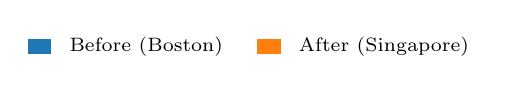
\begin{tikzpicture}
\node[fill=beforeblue, minimum width=3mm, minimum height=2mm, inner sep=0pt] (lb) {};
\node[right=1mm of lb, font=\scriptsize] (lbt) {Before (Boston)};
\node[right=3mm of lbt, fill=afterorange, minimum width=3mm, minimum height=2mm, inner sep=0pt] (la) {};
\node[right=1mm of la, font=\scriptsize] {After (Singapore)};
\end{tikzpicture}\\[0.3ex]
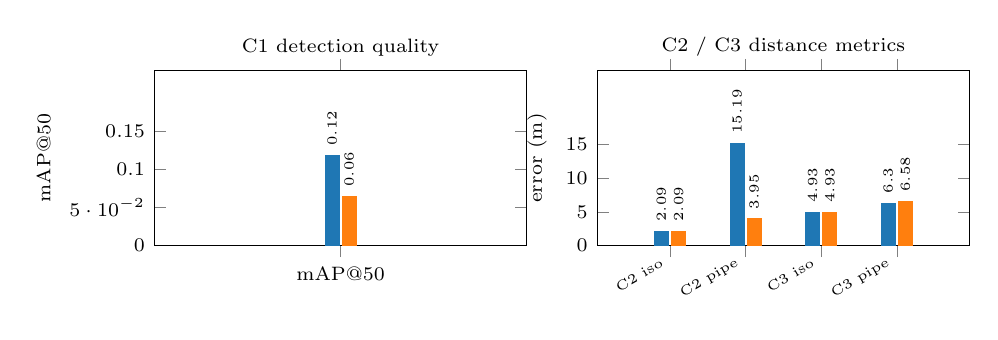
\begin{tikzpicture}
\begin{groupplot}[
  group style={group size=2 by 1, horizontal sep=9mm},
  width=0.52\columnwidth, height=3.8cm,
  ybar=1.2pt, /pgf/bar width=5pt,
  ymin=0, enlarge x limits=0.32,
  tick label style={font=\scriptsize},
  label style={font=\scriptsize},
  title style={font=\scriptsize, yshift=-1ex},
  nodes near coords, nodes near coords style={font=\tiny, rotate=90,
        anchor=west, /pgf/number format/fixed, /pgf/number format/precision=2},
]
\nextgroupplot[title={C1 detection quality},
  ylabel={mAP@50}, symbolic x coords={mAP@50}, xtick=data, ymax=0.23,
  ytick={0,0.05,0.1,0.15}]
\addplot[fill=beforeblue, draw=beforeblue] coordinates {(mAP@50,0.1185)};
\addplot[fill=afterorange, draw=afterorange] coordinates {(mAP@50,0.0644)};
\nextgroupplot[title={C2 / C3 distance metrics},
  ylabel={error (m)}, ymax=26, ytick={0,5,10,15},
  symbolic x coords={C2 iso,C2 pipe,C3 iso,C3 pipe},
  xtick=data, x tick label style={rotate=30, anchor=east, font=\tiny}]
\addplot[fill=beforeblue, draw=beforeblue]
  coordinates {(C2 iso,2.09) (C2 pipe,15.19) (C3 iso,4.93) (C3 pipe,6.30)};
\addplot[fill=afterorange, draw=afterorange]
  coordinates {(C2 iso,2.09) (C2 pipe,3.95) (C3 iso,4.93) (C3 pipe,6.58)};
\end{groupplot}
\end{tikzpicture}
\caption{Reference update on \texttt{singapore\_val}, before versus after:
(a) C1 detection quality, (b) C2/C3 distance metrics.}
\label{fig:tablefull}
\end{figure}

\subsection{Verification of the Isolation Property (F2)}
\label{sec:res-iso}
Before reading any cascade delta, the frozen components must be shown to be
untouched, which is a validity check on the apparatus and not itself a result.
The three isolated-mode rows are exactly zero-delta. C2-isolated minADE is
$2.0899$~m in both runs, and C3-isolated L2 is $0.6900 / 2.4944 / 4.9289$~m at
the three horizons in both runs, to every recorded digit. For deterministic,
parameter-free C2 and C3 fed identical ground-truth inputs, this invariance is
expected by construction, and any nonzero delta would have signalled state or
data leakage between the runs. Its role is to certify that the pipeline-mode
deltas in Table~\ref{tab:results} arise solely from the C1 retraining event,
transmitted through the component interfaces. This exact-equality check held
across all $15$ updates in the campaign.

\subsection{Cascade Concentration at the C1$\to$C2 Interface (F3)}
\looseness=-1
The largest single effect in Table~\ref{tab:results} occurs at the C1$\to$C2
interface. With the Boston-trained C1, C2's pipeline-mode minADE was
$15.1930$~m against an isolated-mode floor of $2.0899$~m, a cascade gap
$\Gamma_2$ of $13.10$~m. This $\Gamma_2$ conflates two sources: C1 detection
error and the loss of velocity information, since C2-isolated uses ground-truth
velocity whereas C2-pipeline uses a zero-velocity rollout
(Section~\ref{sec:setup}); it therefore bounds the combined effect, not
perception error alone. After the Singapore fine-tune, C2-pipeline minADE fell
to $3.9535$~m ($\Gamma_2 = 1.86$~m), a 73.98\% improvement without modifying
C2. The change $\Delta_2 = -11.24$~m is attributable to C1 alone, since the
velocity-information gap is constant across the two runs, so the first
downstream interface dominates the retraining-induced cascade.

\subsection{Non-Monotone Cascade at the System Output (F4)}
The first inversion is at the system output. Even though C2-pipeline improved by
73.98\%, C3-pipeline worsened at every horizon: $+4.25\%$ at 1~s, $+3.01\%$ at
2~s, and $+4.45\%$ at 3~s ($6.2969$~m $\to 6.5770$~m, $\Delta_3 = +0.2801$~m).
The cascade gap at the planner grew from $\Gamma_3 = 1.37$~m to $1.65$~m, with
collision rate zero in both runs. The two pipeline-mode deltas therefore carry
opposite signs: the retraining event that improved the planner's inputs degraded
its output. Read against the diagnostic~\eqref{eq:diag}, the run satisfies the
isolation clause ($\Delta_3^{\text{iso}}=0$) and the degradation clause
($\Delta_3 = +0.28$~m $> \epsilon$) but \emph{not} the upstream-improvement
clause, because aggregate mAP fell (F5). The run is therefore not a clean
instance of entangled enhancement in the strict sense of the base
paper~\cite{wang2024compsac}, which requires $\delta_1 > 0$. It is instead the
related non-monotone regime, in which C2's interface improves while the system
output degrades. It is nonetheless a controlled, quantified instance of the
correction-cascade pattern that the technical-debt literature describes only
qualitatively~\cite{sculley2015hidden}. Fig.~\ref{fig:cascade} illustrates it:
C3-isolated remains fixed at $4.93$~m, since the planner receives identical
ground-truth inputs in both runs, while C3-pipeline drifts from $6.30$ to
$6.58$~m.

\begin{figure}[htbp]
\centering
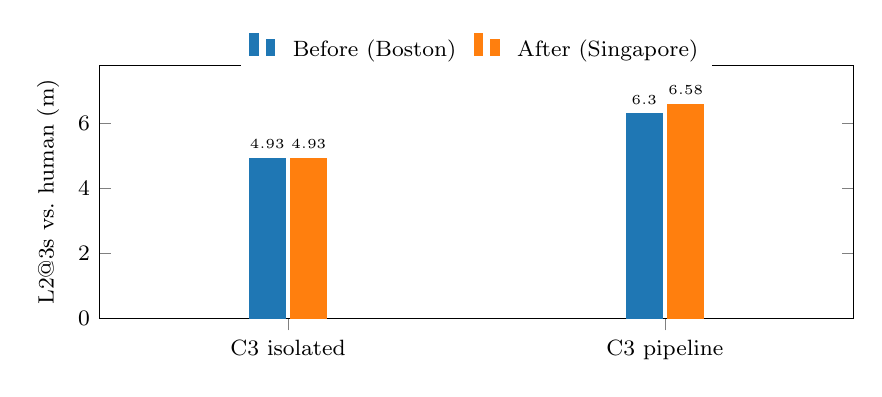
\begin{tikzpicture}
\begin{axis}[
  width=0.92\columnwidth, height=4.8cm,
  ybar=2pt, /pgf/bar width=13pt, ymin=0, ymax=7.8,
  ylabel={L2@3s vs.\ human (m)},
  symbolic x coords={C3 isolated, C3 pipeline}, xtick=data,
  tick label style={font=\footnotesize}, label style={font=\footnotesize},
  enlarge x limits=0.5,
  legend style={at={(0.5,1.15)}, anchor=north, legend columns=2,
                draw=none, font=\footnotesize, column sep=1ex},
  nodes near coords, nodes near coords style={font=\tiny,
        /pgf/number format/fixed, /pgf/number format/precision=2},
]
\addplot[fill=beforeblue, draw=beforeblue]
  coordinates {(C3 isolated,4.93) (C3 pipeline,6.30)};
\addplot[fill=afterorange, draw=afterorange]
  coordinates {(C3 isolated,4.93) (C3 pipeline,6.58)};
\legend{Before (Boston), After (Singapore)}
\end{axis}
\end{tikzpicture}
\caption{Cascade signature on planning: isolated fixed, pipeline drifts.}
\label{fig:cascade}
\end{figure}

\subsection{Aggregate Metric Decoupling at C1 (F5)}
\label{sec:res-decouple}
\looseness=-1
Table~\ref{tab:results} exhibits a second inversion, this one between C1's own
score and the usefulness of its outputs. The Singapore-fine-tuned C1, the
checkpoint that improved C2 by 74\%, scores \emph{lower} on its own aggregate
validation metric than its Boston-trained predecessor (mAP@50 $0.1185 \to
0.0644$, $-45.66\%$; recall $0.0866 \to 0.0477$). The immediate cause is
small-data overfitting: the Singapore fine-tune set contains only 119 images
(944 instances) with a sparse class mix, and the fine-tuned detector converges
to detection regimes that diverge from the validation label distribution, as
evident in the confusion matrix of Fig.~\ref{fig:confusion}, where most non-car
classes collapse into the background row. The cascade, however, does not
propagate through the aggregate score but through the detection outputs
themselves: a detector can lose mAP while emitting outputs that are more useful
to its downstream consumer on the relevant scenes. Aggregate component metrics
and interface behavior therefore decouple, here moving in opposite directions
with large magnitudes on both sides, so a component's own metric is not a
reliable admission criterion. This is the per-component, system-scale analogue
of the negative-flip phenomenon reported for classifier
updates~\cite{yan2021pctraining}.

\begin{figure}[htbp]
\centering
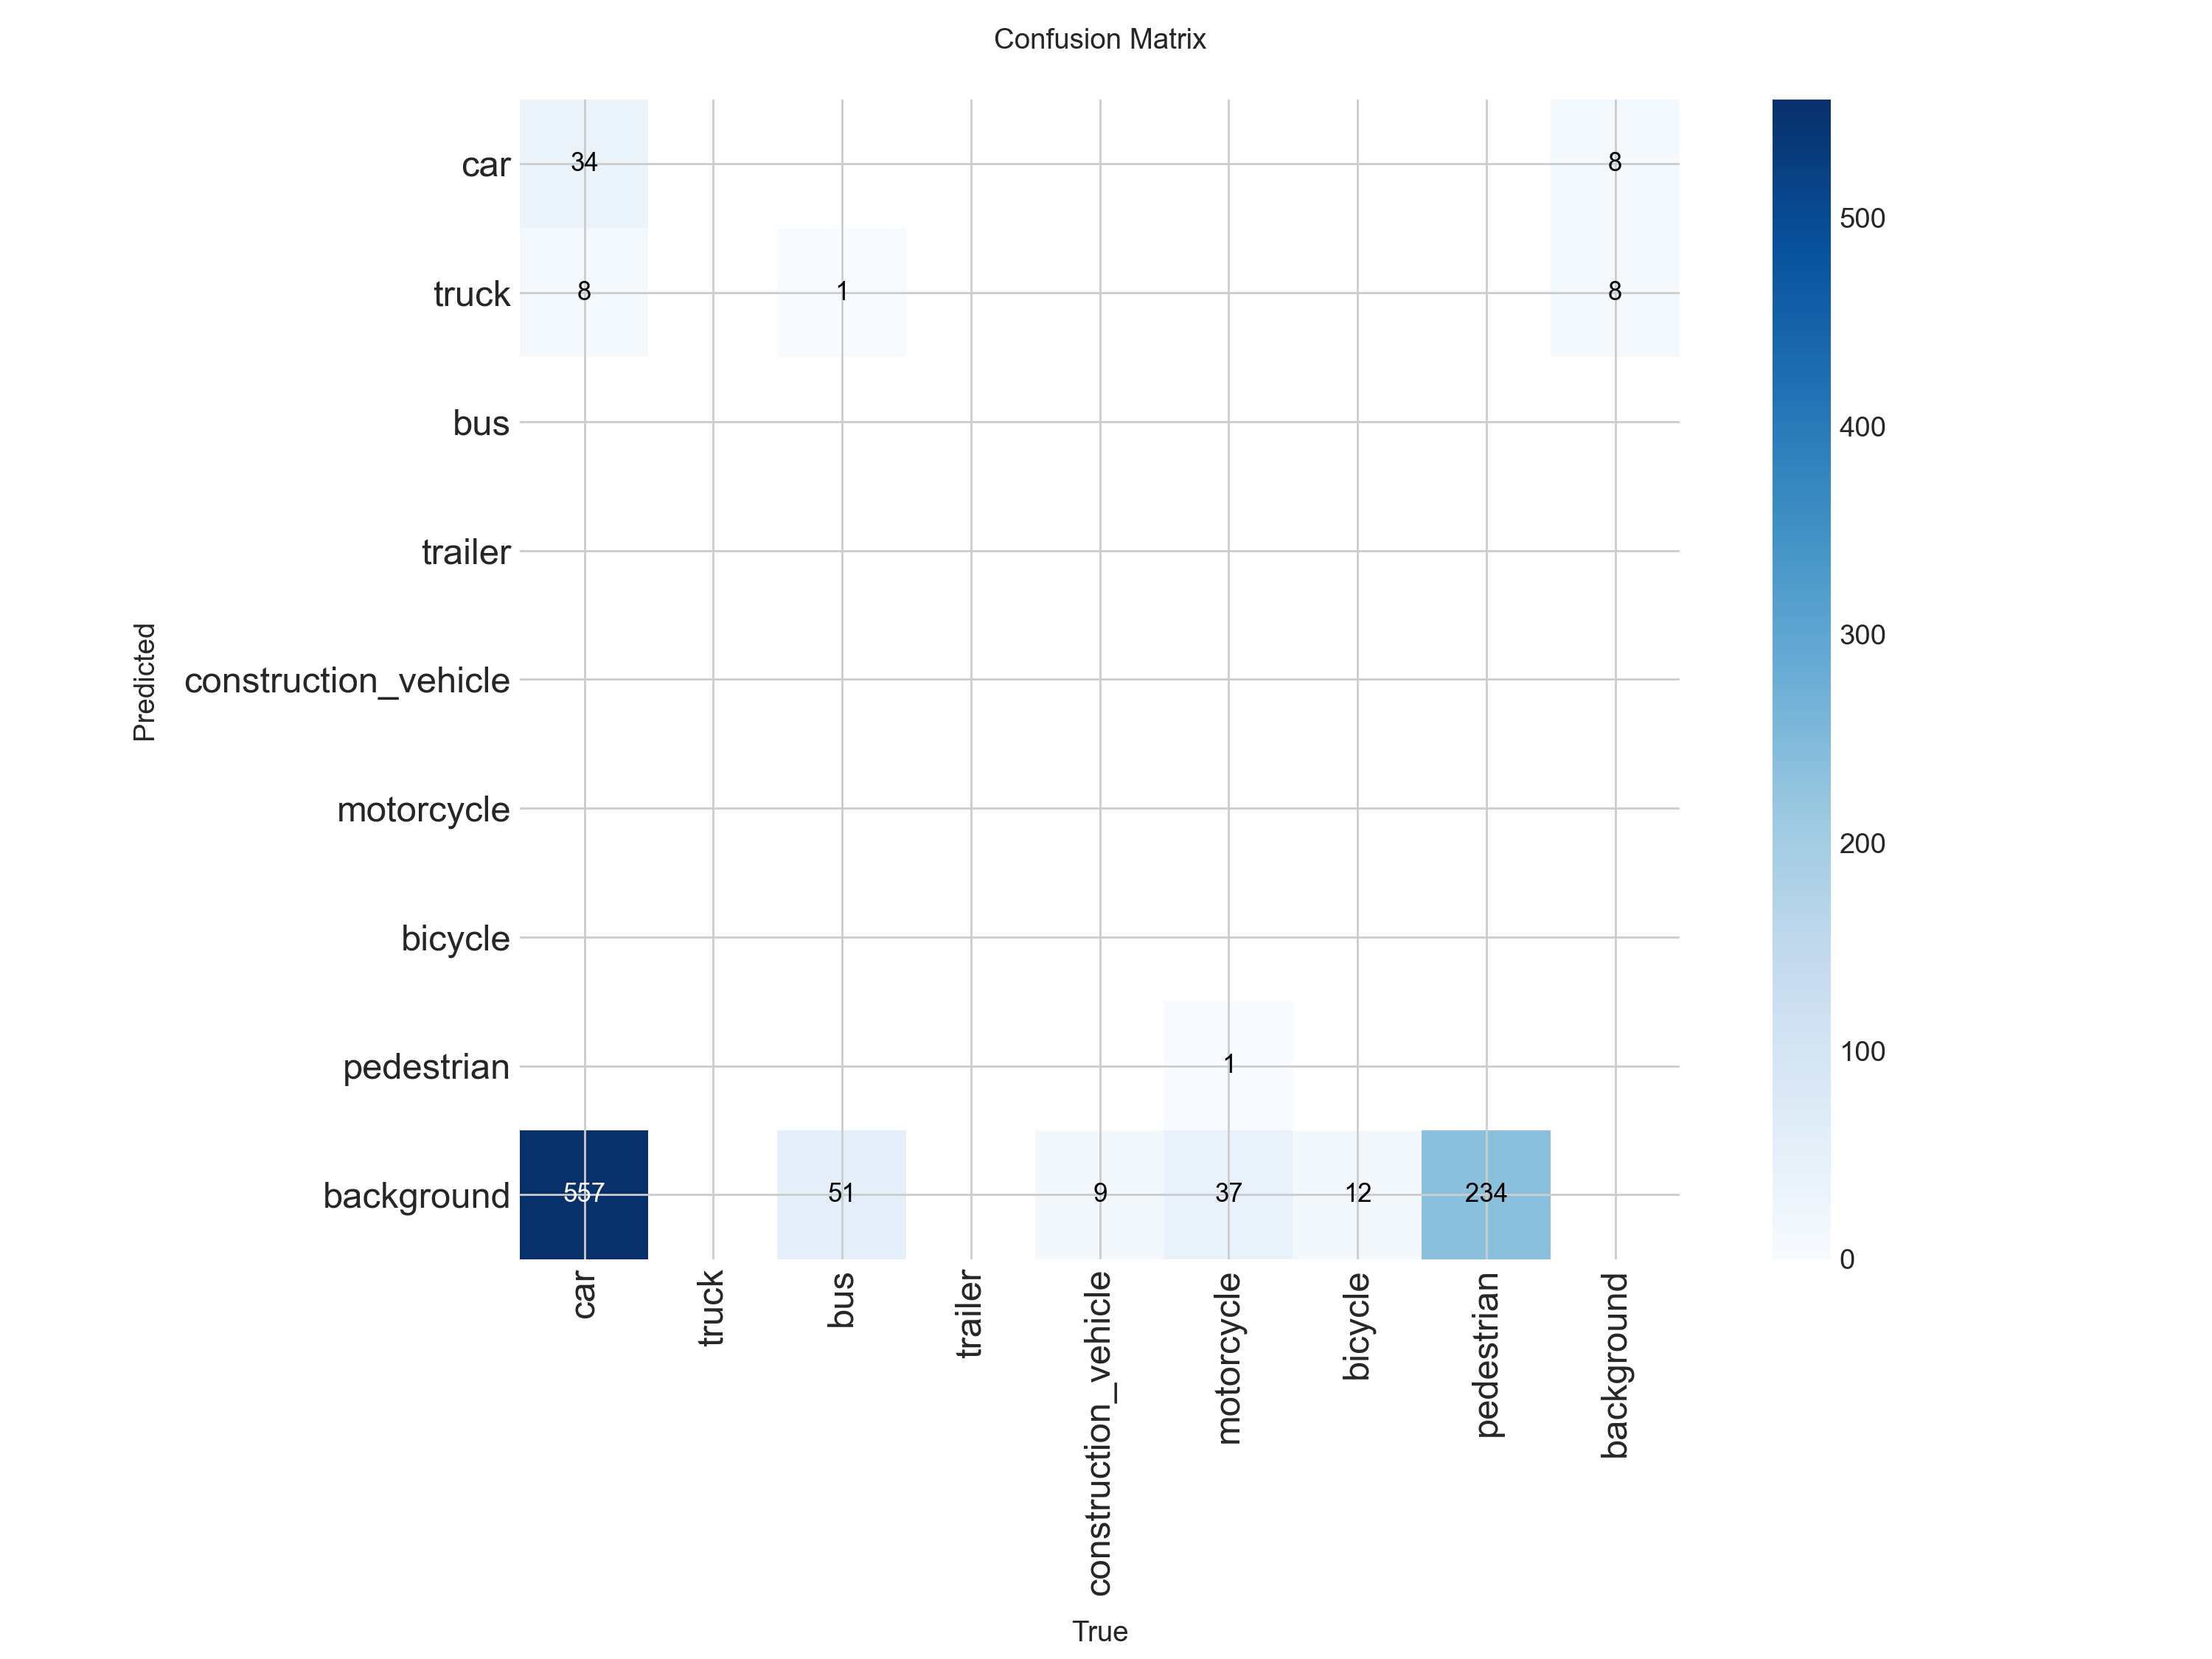
\includegraphics[width=0.92\columnwidth]{figures/fig05_singapore_confusion.png}
\caption{Confusion matrix of the Singapore-fine-tuned $C_1$.}
\label{fig:confusion}
\end{figure}

\subsection{The Campaign: A Landscape, Not a Constant (F6)}
\label{sec:res-campaign}
The reference update is a single point in this space.
Table~\ref{tab:campaign} reports all $15$ updates of the campaign
(Section~\ref{sec:campaign}), and three patterns emerge.

First, the cascade is always present, but its magnitude varies substantially.
The plan shift, defined as the distance the planned path moves when the incumbent
C1 is replaced by the retrained one, ranges from $1.33$~m to $7.80$~m. The same
form of retraining alters the driving decision only slightly in one campaign and
substantially in another, so no single number summarizes the entanglement.

Second, the direction of the terminal effect is campaign-dependent. In the
reference update the planner regressed, but across the $15$ updates $\Delta_3 >
0$ (planner worse) in $11$ and $\Delta_3 < 0$ in $4$. Two of the latter are
material improvements of $0.20$ and $1.04$~m, both from small-data (quarter)
updates, while the other two are negligible at under a millimetre and are
labelled benign in Table~\ref{tab:campaign}. The reference conclusion that
retraining degrades the planner therefore does not hold universally.

Third, the amount of fine-tuning data governs the magnitude. Averaging the
$10$-epoch updates by data size, the mean plan shift is $6.12$~m for the full
set, $2.98$~m for half, and $3.46$~m for a quarter, so the full-data updates
produce the largest and most variable downstream change. A detector that adapts
more strongly to the new city induces a larger change throughout the pipeline.
Across all $15$ updates $\delta_1 < 0$ (Table~\ref{tab:campaign}), which is the
small-data effect of F5, so this campaign realizes the decoupling and
non-monotone regimes repeatedly ($4$ updates match the reference decoupling
pattern of $\delta_1<0$ with $\Delta_2<0$, and $2$ are essentially benign) but
not the strict entangled enhancement of~\eqref{eq:ee}, which requires $\delta_1 >
0$. Section~\ref{sec:res-balanced} removes exactly that obstacle.

\begin{table}[htbp]
\caption{The $15$-update retraining campaign on \texttt{singapore\_val}.
$\delta_1$: detector-score change (positive better); $\Delta_2$:
prediction-error change (negative better); $\Delta_3$: planner-error change
(negative better); shift: plan shift in metres.}
\label{tab:campaign}
\centering
\renewcommand{\arraystretch}{1.15}
\setlength{\tabcolsep}{3.5pt}
\footnotesize
\begin{tabular}{@{}lrrrrrl@{}}
\toprule
\textbf{Update} & \textbf{img} & \textbf{$\delta_1$} & \textbf{$\Delta_2$} & \textbf{$\Delta_3$} & \textbf{shift} & \textbf{regime} \\
\midrule
Full, 10\,ep, s1      & 119 & $-0.022$ & $+5.39$ & $+0.68$ & $7.80$ & other \\
Full, 10\,ep, s2      & 119 & $-0.022$ & $-1.02$ & $+1.34$ & $7.40$ & decoupling \\
Full, 10\,ep, s3      & 119 & $-0.025$ & $-2.23$ & $+0.26$ & $3.17$ & decoupling \\
Half, 10\,ep, s1      &  60 & $-0.053$ & $+2.38$ & $+0.26$ & $3.17$ & other \\
Half, 10\,ep, s2      &  60 & $-0.044$ & $+1.63$ & $+0.26$ & $3.17$ & other \\
Half, 10\,ep, s3      &  60 & $-0.045$ & $+2.17$ & $+0.24$ & $2.59$ & other \\
Quarter, 10\,ep, s1   &  30 & $-0.060$ & $+1.83$ & $+0.26$ & $3.17$ & other \\
Quarter, 10\,ep, s2   &  30 & $-0.057$ & $-5.29$ & $-0.20$ & $3.29$ & decoupling \\
Quarter, 10\,ep, s3   &  30 & $-0.066$ & $-3.85$ & $-1.04$ & $3.93$ & decoupling \\
Full, 5\,ep, s1       & 119 & $-0.037$ & $+2.32$ & $+0.24$ & $2.59$ & other \\
Full, 5\,ep, s2       & 119 & $-0.052$ & $+0.83$ & $-0.00$ & $1.33$ & benign \\
Full, 5\,ep, s3       & 119 & $-0.052$ & $+0.83$ & $-0.00$ & $1.33$ & benign \\
Full, 20\,ep, s1      & 119 & $-0.033$ & $+8.00$ & $+0.24$ & $2.59$ & other \\
Full, 20\,ep, s2      & 119 & $-0.006$ & $+9.38$ & $+0.26$ & $3.17$ & other \\
Full, 20\,ep, s3      & 119 & $-0.017$ & $+2.42$ & $+0.26$ & $3.17$ & other \\
\bottomrule
\end{tabular}
\end{table}

\subsection{Strict Entangled Enhancement Under Class-Balanced
Retraining (F7)}
\label{sec:res-balanced}
Every update in Table~\ref{tab:campaign} lost detector accuracy, and the cause is
the class mix rather than the cascade: the $119$-image Singapore set is dominated
by \texttt{car}, so a small fine-tune overfits that class and the aggregate mAP
falls. Because the strict condition~\eqref{eq:ee} requires $\delta_1 > 0$, this
small-data artifact, and not the pipeline, is what stood between the campaign and
a textbook instance of entangled enhancement.

We therefore repeat the retraining with a class-balanced training split. Images
containing rare classes are oversampled so that the per-class instance
distribution flattens, with a repeat factor $(n_{\max}/n_c)^{p}$ per class $c$
clipped to $[1,12]$. The validation split is left untouched, so mAP stays
comparable to every other run in this paper. At $p{=}0.5$ the split grows from
$119$ to $399$ images and the max/min class ratio falls from $34.8$ to $17.7$. We
run two balance strengths ($p \in \{0.5, 1.0\}$), two training lengths
($10$ and $20$ epochs), and three seeds, giving $12$ updates.

The balancing achieves its purpose. The detector now \emph{improves} on its own
metric in $6$ of the $12$ updates, reversing the sign of $\delta_1$ that held
throughout Table~\ref{tab:campaign}. More importantly, three of those updates
also degrade the planner, which is exactly the strict entangled-enhancement
condition~\eqref{eq:ee}: C1 gets better on its own terms while the system it
feeds gets worse. Table~\ref{tab:balanced} lists them together with a
representative counter-example. All three arise at $20$ epochs, under both
balance strengths and across two seeds, so the effect is not a single lucky run.
Longer adaptation is what lifts C1 past the incumbent, and it is precisely in
that regime that the downstream cost appears.

\begin{table}[htbp]
\caption{Class-balanced updates. The first three satisfy the strict
condition~\eqref{eq:ee}: $\delta_1>0$ (C1 improves) with $\Delta_3>0$ (system
degrades). Full matrix: $\delta_1>0$ in $6/12$, strict EE in $3/12$.}
\label{tab:balanced}
\centering
\renewcommand{\arraystretch}{1.15}
\setlength{\tabcolsep}{4pt}
\footnotesize
\begin{tabular}{@{}lrrrrc@{}}
\toprule
\textbf{Update} & \textbf{$\delta_1$} & \textbf{$\Delta_2$} & \textbf{$\Delta_3$} & \textbf{shift} & \textbf{strict EE} \\
\midrule
$p{=}0.5$, 20\,ep, s1 & $+0.031$ & $+3.87$ & $+0.24$ & $2.59$ & \textbf{yes} \\
$p{=}1.0$, 20\,ep, s3 & $+0.021$ & $+8.59$ & $+0.24$ & $2.59$ & \textbf{yes} \\
$p{=}1.0$, 20\,ep, s2 & $+0.012$ & $+0.88$ & $+0.24$ & $1.26$ & \textbf{yes} \\
\midrule
$p{=}1.0$, 10\,ep, s2 & $+0.002$ & $-7.70$ & $-0.63$ & $4.67$ & no \\
\bottomrule
\end{tabular}
\end{table}

This is the paper's central empirical claim. Entangled enhancement is not only an
analytically modeled hazard~\cite{wang2024compsac}; it occurs in a real
perception--prediction--planning pipeline, and it is reachable by an ordinary
maintenance action, namely retraining one component on new-city data with a
balanced class mix. It also sharpens the practical warning: the three strict
cases would each have passed a component-level review, because C1's own metric
improved, yet each made the driving output worse.

\subsection{Evaluation of CARA's Drift Screen (F6 continued)}
\label{sec:res-gate}
The campaign enables an evaluation of the interface-drift front-end of CARA
(Section~\ref{sec:cara-frontend}) as a predictor of risk. For each of the $15$
updates we compute the drift score of the retrained detector against the
incumbent on the audit scenes and assess how well it anticipates the downstream
disruption that only the full pipeline reveals.

Ranked against the plan shift each update caused, the drift score is a real but
loose predictor. The rank correlation between drift and plan shift is
$\approx 0.41$, and Fig.~\ref{fig:drift-scatter} shows the relationship. The
agreement is clearest at the extremes: the two updates with the largest plan
shifts ($7.80$ and $7.40$~m) also carry the two highest drift scores, and drift
follows the same data-size trend as plan shift. The front-end therefore carries
usable signal about which updates disturb the plan, although it is far from a
precise predictor and is best used to prioritize updates for the full assessment
rather than as a standalone decision.

\begin{figure}[htbp]
\centering
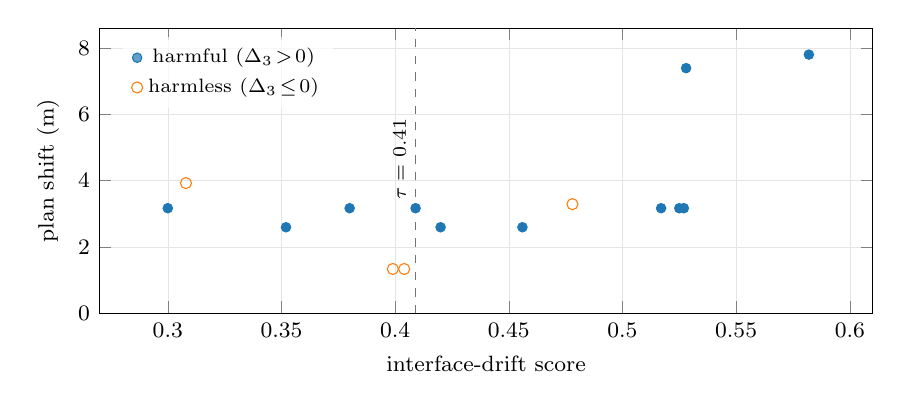
\begin{tikzpicture}
\begin{axis}[
  width=0.94\columnwidth, height=5.2cm,
  xlabel={interface-drift score}, ylabel={plan shift (m)},
  xmin=0.27, xmax=0.61, ymin=0, ymax=8.6,
  tick label style={font=\footnotesize}, label style={font=\footnotesize},
  legend style={at={(0.03,0.97)}, anchor=north west, font=\scriptsize,
                draw=none, fill=white, fill opacity=0.7, text opacity=1},
  grid=both, grid style={line width=0.2pt, draw=gray!20},
]
% harmful updates (Delta3>0): filled circles
\addplot[only marks, mark=*, mark size=1.7pt, beforeblue] coordinates {
  (0.582,7.804) (0.528,7.395) (0.527,3.167) (0.300,3.167) (0.409,3.167)
  (0.420,2.592) (0.380,3.167) (0.352,2.592) (0.456,2.592) (0.525,3.167)
  (0.517,3.167)};
% harmless updates (Delta3<=0): open circles
\addplot[only marks, mark=o, mark size=2pt, afterorange] coordinates {
  (0.478,3.289) (0.308,3.925) (0.404,1.333) (0.399,1.333)};
% balanced admission threshold
\draw[dashed, black!55] (axis cs:0.409,0) -- (axis cs:0.409,8.6);
\node[font=\scriptsize, anchor=south, rotate=90] at (axis cs:0.409,4.6)
  {\,$\tau=0.41$};
\legend{harmful ($\Delta_3\!>\!0$), harmless ($\Delta_3\!\le\!0$)}
\end{axis}
\end{tikzpicture}
\caption{Interface drift vs.\ plan shift over the $15$ updates
(Spearman $\approx 0.41$); dashed line is the balanced threshold.}
\label{fig:drift-scatter}
\end{figure}

\subsection{Evaluation of CARA's Admission Rule}
\label{sec:res-admission}
We next evaluate the drift score as the binary admit/hold rule of CARA's
front-end, scored against ground truth. We label an update ``harmful'' when it
actually worsened the planner ($\Delta_3 > 0$); of the $15$ updates, $11$ are
harmful and $4$ are not. Treated as a ranking, the drift score places a harmful
update above a harmless one about $70\%$ of the time (AUROC $\approx 0.70$),
consistent with the loose rank correlation above.

As a thresholded decision the rule is sensitive to the threshold, as
Table~\ref{tab:admission} shows. At a strict threshold every one of the $15$
updates drifts enough to be held, so no harmful update is admitted (recall $1.0$)
but no update is admitted at all (specificity $0$), which is safe but provides no
discrimination. Relaxing the threshold to a balanced operating point yields a
genuinely selective rule: it catches roughly three-quarters of the harmful
updates (recall $0.73$) while correctly admitting three-quarters of the harmless
ones (specificity $0.75$), at precision $0.89$. None of the $15$ retrained
pipelines produced a collision, so the collision-rate-aware clause of
Algorithm~\ref{alg:cara} could not be exercised on this data, and the terminal-L2
clause carries the decision alone.

\begin{table}[htbp]
\caption{CARA drift-rule decisions against ground truth ($\Delta_3 > 0 =$
harmful). Confusion counts are (held-harmful, held-harmless, admitted-harmful,
admitted-harmless).}
\label{tab:admission}
\centering
\renewcommand{\arraystretch}{1.2}
\setlength{\tabcolsep}{5pt}
\begin{tabular}{@{}lcccccc@{}}
\toprule
\textbf{Threshold} & \textbf{TP/FP/FN/TN} & \textbf{Rec.} & \textbf{Spec.} & \textbf{Prec.} & \textbf{F1} \\
\midrule
Strict ($\tau{=}0.25$)   & $11/4/0/0$ & $1.00$ & $0.00$ & $0.73$ & $0.85$ \\
Balanced ($\tau{=}0.41$) & $8/1/3/3$  & $0.73$ & $0.75$ & $0.89$ & $0.80$ \\
\bottomrule
\end{tabular}
\end{table}

We interpret these results conservatively. CARA's low-cost front-end works in
principle on our data but is not a validated rule, because the discriminating
threshold was chosen on the same $15$ points against which it is judged, with no
held-out set, and with only three audit scenes the evaluation constitutes a proof
of concept. The full admission procedure of Algorithm~\ref{alg:cara}, which runs
the complete dual-mode profile rather than the drift proxy, is the more reliable
decision, and the front-end serves as its low-cost first filter. We report the
front-end evaluation because it is what the $15$-update campaign can support at
this scale.

\subsection{Training Diagnostics}
Both fine-tunes converged within their epoch budgets with monotone loss
decay, as Fig.~\ref{fig:curves} shows for the Boston run: the box,
classification, and distribution-focal losses decrease on both the train and
validation splits, while precision, recall, and mAP@50 increase, with mAP@50
rising from $0.039$ at epoch 1 to $0.119$ at epoch 10. Each fine-tune completes
in under a GPU-minute, several orders of magnitude below the cost of a single
E2E training run~\cite{sun2024sparsedrive}, which is what renders a campaign of
repeated retraining feasible. The cascade propagates through the ego-frame
positions of the detected boxes, which alter the forecasts and hence the plan,
independently of whether the detections differ visibly to the eye.

\begin{figure}[htbp]
\centering
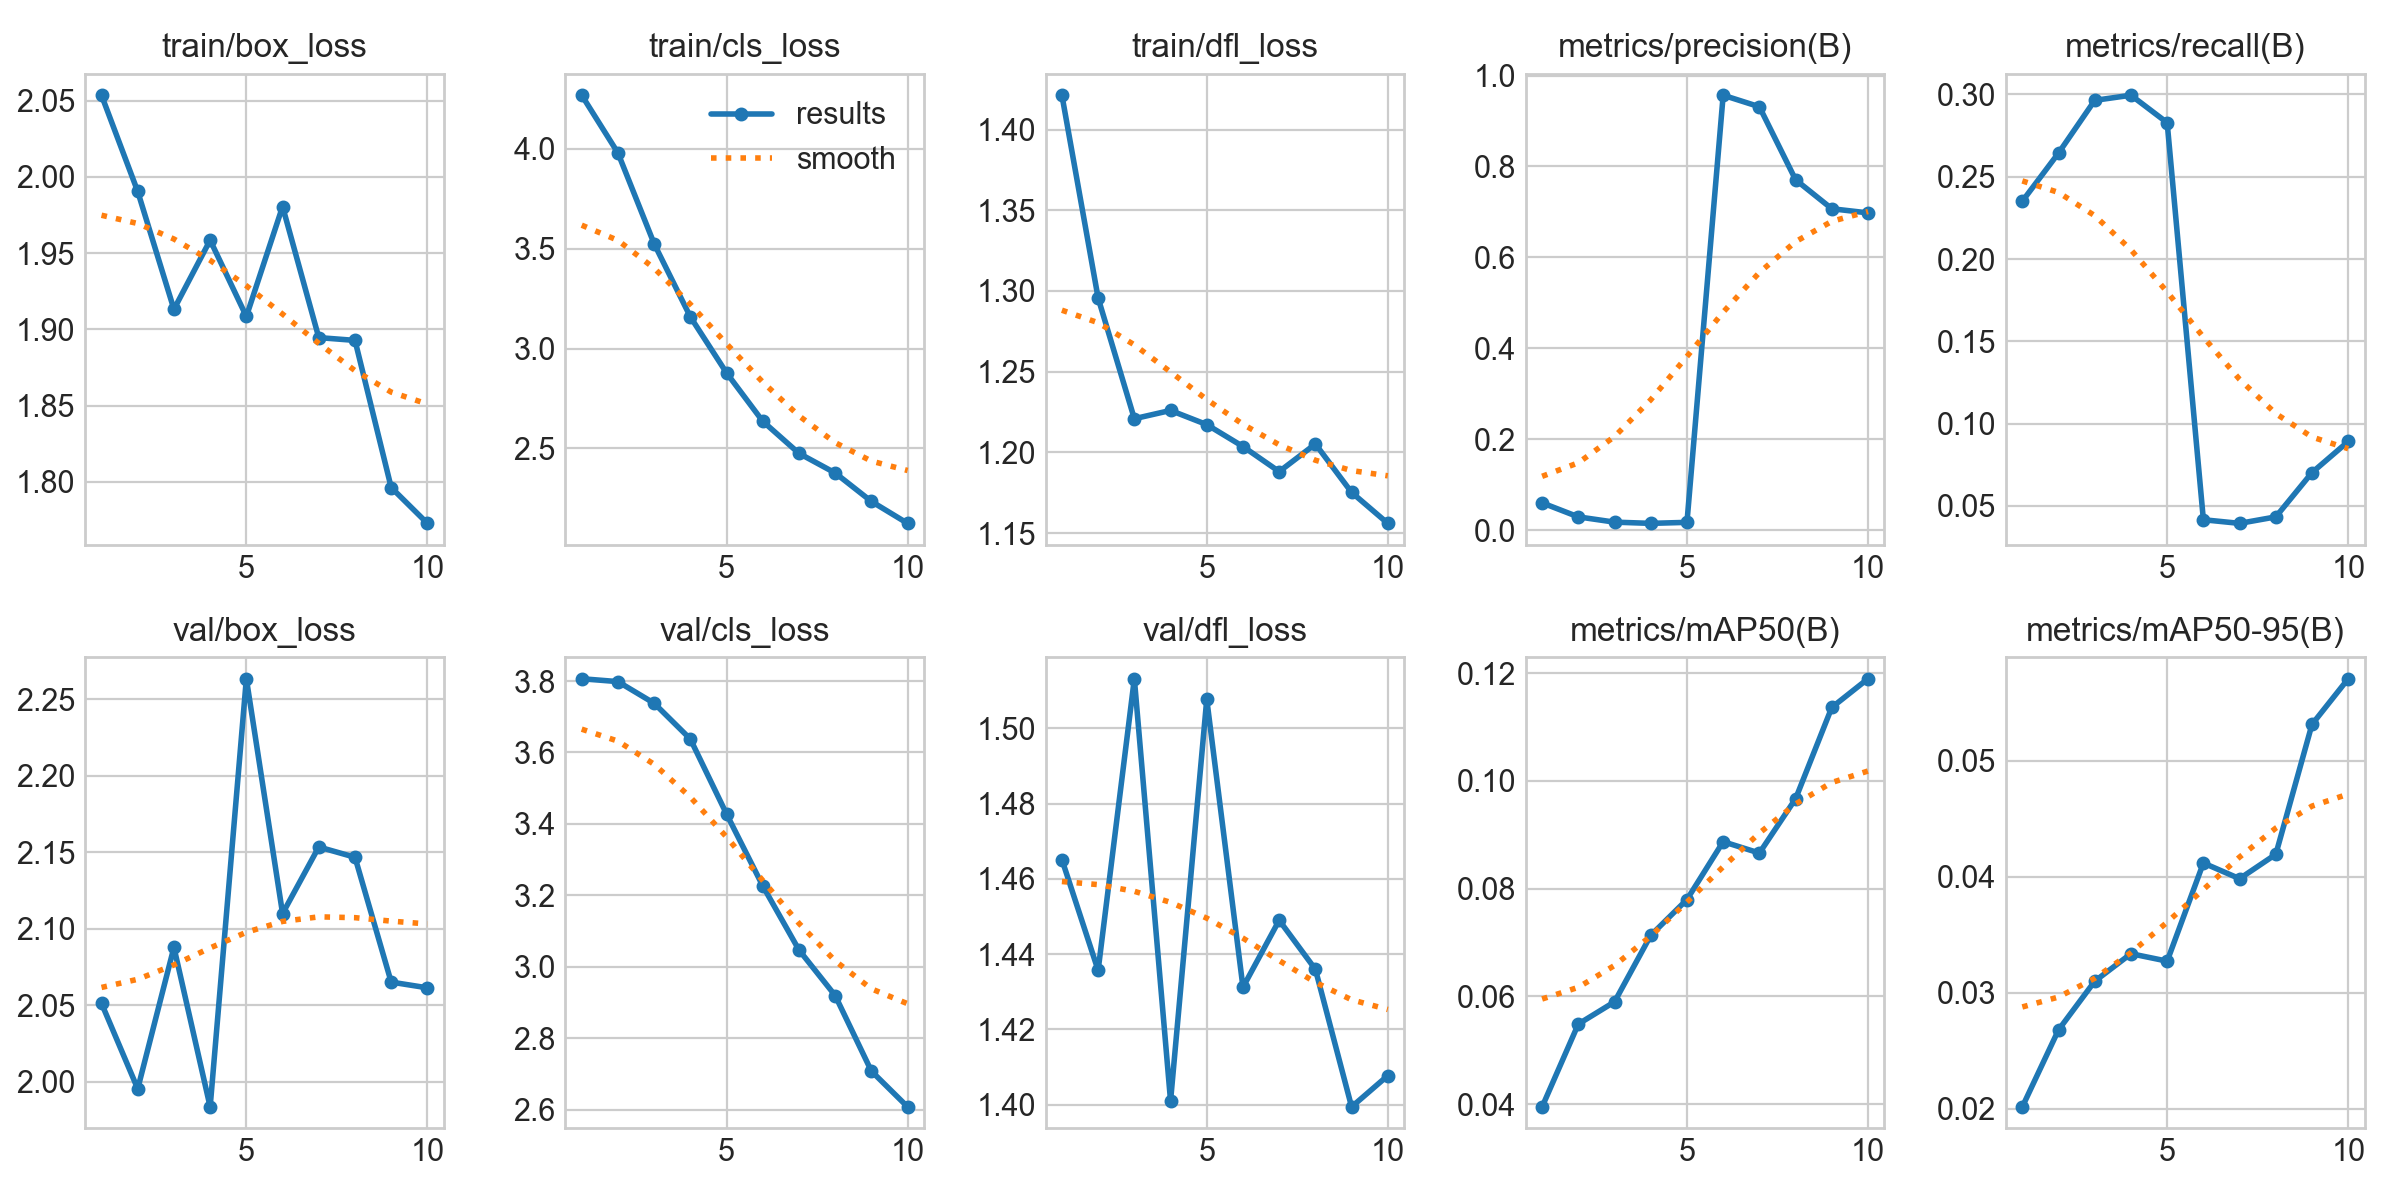
\includegraphics[width=\columnwidth]{figures/fig04_boston_curves.png}
\caption{YOLOv11n $C_1$ Boston fine-tune training curves.}
\label{fig:curves}
\end{figure}

% ============================================================================
\section{Discussion}
\label{sec:implications}
% ============================================================================
We explain the mechanism behind the non-monotone cascade, place CARA among
related maintenance techniques, and state the threats to validity.

\subsection{Why the Cascade Is Non-Monotone}
Under the Boston-trained C1, the planner's inputs were substantially displaced
($\Gamma_2 = 13.10$~m) in a regime whose errors the proposal-and-score rules
absorbed: missed or grossly misplaced agents leave the proximity penalty
inactive, so the planner follows its kinematic prior, which on these scenes
approximated the human trajectory. The fine-tuned C1 relocated detections near
their true positions and re-activated the penalty with correctly anchored but
coarse (zero-velocity) forecasts, causing the planner to react to obstacles it
had previously ignored. Downstream components can thus absorb upstream error,
and, symmetrically, upstream improvement can expose masked downstream
sensitivity. A retrained component therefore cannot be admitted on its own
interface alone.

\looseness=-1
This mechanism also cautions against a literal interpretation of the terminal
metric. Collision rate was zero before and after in every update, and the higher
L2 of the reference case arises because the improved detector caused the planner
to react to real agents rather than follow a kinematic prior that happened to
track the recorded human path. This is the ego-forecasting shortcut of nuScenes open-loop
L2, under which perception-agnostic prediction is
competitive~\cite{zhai2023rethinking} and open-loop error is weakly tied to
closed-loop quality~\cite{codevilla2018offline}. A regression on this metric may
therefore mark a \emph{safer} planner that scores worse on a measure rewarding
ignored perception, so the terminal readings here should be read as reduced
trajectory agreement, not an established safety regression, and a closed-loop or
NAVSIM-style metric~\cite{dauner2024navsim} is the appropriate safeguard.

\subsection{CARA Among Related Maintenance Techniques}
The findings give three maintenance rules that CARA (Section~\ref{sec:cara})
enforces directly. An update must not be admitted on the retrained component's
own metric, because of the decoupling in F5 and, most directly, the strict cases
of F7 in which C1 improved while the system degraded.
Admission must not stop at the first interface, because the non-monotone cascade
of F4 lets an improvement at C2 coincide with a regression at C3. And because the
downstream effect is a landscape (F6) rather than a constant, a maintenance
policy should assess several candidate updates rather than trust one.

CARA is one of several complementary techniques for these rules, not a
replacement for them. Regression-constrained retraining such as
positive-congruent training~\cite{yan2021pctraining} and backward-compatible
training~\cite{shen2020bct} \emph{reduces} the cascade at its source by
constraining the update. Uncertainty-propagating
interfaces~\cite{ivanovic2022propagating} \emph{absorb} the residual by passing
distributions instead of point estimates across the perception--prediction
boundary. Between-stage data validation~\cite{breck2019data} \emph{monitors} the
interface in production. CARA adds the missing \emph{admission} step that measures
the downstream cascade directly before an update is deployed, and its low-cost
interface-drift front-end (Section~\ref{sec:cara-frontend}) can operate alongside
the same production monitors.

% ============================================================================
\section{Related Work}
\label{sec:related}
% ============================================================================

\subsection{End-to-End Driving and Its Maintenance Limits}
UniAD put detection, tracking, mapping, motion forecasting, occupancy
prediction, and planning into a single planning-oriented
network~\cite{hu2023uniad}. VAD replaced dense rasterized scene
representations with vectorized ones for efficiency~\cite{jiang2023vad}.
SparseDrive introduced fully sparse scene representations and reported the
resource profile of the flagship systems: $7.2\times$ faster training and
$5\times$ faster inference than UniAD, whose training takes about 144
GPU-hours~\cite{sun2024sparsedrive}. The main survey of the field lists
interpretability, causal confusion, and robustness under distribution shift
as open challenges, and it does not treat component-level maintenance or
retraining policy at all~\cite{chen2024e2esurvey}.

A recent E2E repair literature addresses maintenance directly. CorrectAD
builds a self-correction loop that diagnoses failures, generates targeted
training video with a diffusion model, and fine-tunes the entire E2E planner
on old plus new data, correcting 62.5\% of failure cases on
nuScenes~\cite{ma2025correctad}. R2SE avoids full-model retraining by freezing
the generalist model and training reinforcement-learned low-rank adapter
specialists on failure regions, motivated by the catastrophic forgetting that
naive fine-tuning causes~\cite{liu2025r2se}. Both reintroduce modular structure
to make maintenance tractable, motivating the modular architecture adopted in
this work.

\subsection{Evaluation of Driving Systems}
Our planning metric is open-loop displacement error on nuScenes, and the
limits of this protocol are well documented. Codevilla et al. showed as early
as 2018 that offline prediction error correlates only weakly with actual
closed-loop driving quality~\cite{codevilla2018offline}. Zhai et al. found
that a trivial MLP using only ego state, with no perception at all, matches
perception-based E2E methods on nuScenes open-loop
L2~\cite{zhai2023rethinking}. Dauner et al. showed that open-loop
ego-forecasting and closed-loop driving are misaligned tasks, and that a
largely rule-based planner, PDM-Closed, outperformed learned
planners~\cite{dauner2023parting}. Their later NAVSIM benchmark provides
short-horizon non-reactive metrics that align far better with closed-loop
performance~\cite{dauner2024navsim}. These critiques target open-loop metrics
used to \emph{rank} architectures; our use is differential (the same frozen
planner, same scenes, one upstream change), so much of that weakness cancels,
and we report collision rate alongside L2 and revisit the caveat in
Section~\ref{sec:implications}.

\subsection{Model Updates, Regression, and Interface Compatibility}
What we measure at system scale has per-sample analogues in the model-update
literature. Yan et al. showed that model updates cause negative flips, samples
the old model handled correctly that the new model gets wrong, at rates of
4--5\% even between equal-accuracy retrains of identical architectures, and
they proposed positive-congruent training with focal distillation to suppress
them~\cite{yan2021pctraining}. The backward-compatible training of Shen et al.
constrains a new upstream representation model so that unchanged downstream
consumers keep working~\cite{shen2020bct}, which is the same situation as
updating C1 beneath a frozen C2 and C3. On the monitoring side, the data
validation system of Breck et al. runs two-sample distribution tests between
pipeline stages in production~\cite{breck2019data}. On a nuScenes
detector--tracker--predictor stack nearly the same shape as ours, Ivanovic et
al. showed that propagating state uncertainty across the
perception--prediction interface, instead of passing point estimates, improves
forecasting by a wide margin~\cite{ivanovic2022propagating}. These works
provide mitigation techniques. This paper contributes the complementary
controlled measurement of the cascade that such techniques are intended to
mitigate.

\subsection{Reliability Modeling of Machine Learning Systems}
The technical-debt analysis of Sculley et al. introduced CACE, unstable data
dependencies, and correction cascades as qualitative failure modes of ML
systems~\cite{sculley2015hidden}. The base paper for this work, Wang and
Machida~\cite{wang2024compsac}, formalized imperfect retraining of a
two-component MLS as a continuous-time Markov chain, named entangled
enhancement, and compared progressive and conservative maintenance policies.
Their follow-on work casts the same problem as an availability--continuity
trade-off~\cite{wang2025issre}. Both are analytical models whose state space
grows as $2^N$ for $N$ components, and both are calibrated on synthetic
transition rates. This paper provides an empirical counterpart: the isolation
property we verify (F2) is the property their state factorization assumes, and
the coupling factor we propose (Section~\ref{sec:cara}) is a measured statistic
that can replace those synthetic rates.

% ============================================================================
\section{Conclusion}
\label{sec:conclusion}
% ============================================================================
We presented a controlled study of single-component retraining in a modular
perception--prediction--planning pipeline under a geographic domain shift. Using
dual-mode evaluation with a verified isolation control, and running a campaign of
$15$ retraining updates rather than a single event, we found that retraining C1
alone reliably disturbs the downstream plan, but by an amount that is not a
constant. The plan shift ranges from $1.33$ to $7.80$~m, the planner is hurt by
most updates yet helped by a few, and the effect grows with fine-tuning data. In
the reference update C1's aggregate metric moved opposite to its interface
usefulness, and the same decoupling and non-monotone regimes recur across the
campaign. A further $12$ updates with a class-balanced training split then
delivered the effect in its strict form: with the small-data accuracy penalty
removed, $\delta_1$ turned positive in half of the updates, and in three of them
the planner degraded at the same time. Entangled enhancement is therefore not
only an analytically modeled hazard but an observable one in a real driving
pipeline. Together these results show that component-level validation is
insufficient for safe MLS maintenance, since each of those three updates would
have passed a review of C1 alone. We proposed the CARA admission method for
maintaining such pipelines and evaluated its interface-drift front-end, which
carries a real but imperfect signal (AUROC $\approx 0.70$) and is best used to
prioritize updates rather than to decide on them. The broader contribution is
methodological: cascade effects can be measured under exact controls, but only in
an architecture that exposes its interfaces.

\bibliographystyle{IEEEtran}
\bibliography{references}
\end{document}
